\documentclass{article}
% \documentclass[draft,linenumbers]{agujournal}

\usepackage{appendix}
\usepackage{pifont}
\usepackage{subfigure}
\usepackage[utf8]{inputenc}
\usepackage{CJK}
\usepackage{amsmath}
\usepackage{graphicx}
\usepackage{bm}
\usepackage{etoolbox}
\usepackage{float}
\usepackage{lineno}
\usepackage{color}
\usepackage{booktabs}
\usepackage{array}
\usepackage{graphicx,subfigure}
\usepackage{multirow}
\usepackage{algpseudocode}
\usepackage[linesnumbered,ruled]{algorithm2e}
\usepackage{hyperref}
\usepackage{authblk}
\def\CO2{CO\textsubscript{2}}
\def\N2{N\textsubscript{2}}

\title{The user manual of StrataTrapper software}

\author[1]{Senyou An}
\author[1]{Nele Wenck}
\author[1]{Ann Muggeridge}
\author[1]{\href{mailto:s.krevor@imperial.ac.uk}{Samuel Krevor}}

\affil[1]{Department of Earth Science and Engineering, Imperial College London, London, SW7 2AZ, UK}

\begin{document}
\maketitle

\begin{abstract}
    Accurately considering the heterogeneity, particularly the capillary pressure heterogeneity, in reservoir characterisation, which will be further utilized for  multiphase flow simulation.
\end{abstract}


\section{Introduction}

In StrataTrapper we translate cutting edge research on the geological fluid dynamics and trapping of \CO2 into innovative characterisation and modelling software tools that will be used by industry to reduce risks and costs of \CO2 storage projects. The tools will be commercialised through incorporation into the \CO2 reservoir simulation platform OpenGoSim, in addition to being made open-source. We will demonstrate the applicability of these tools to the Endurance field in the Southern North Sea and the East Mey Site in the Central and Northern North Sea. The result of the work will be the commercialisation of the StrataTrapper reservoir simulation tools for the rapid screening, risking, project design, and management of \CO2 storage.

Reservoir simulations of injected \CO2 plumes are central to the successful engineering and management of \CO2 storage. Plume migration rates and direction determine the storage efficiency and significance of potential leakage pathways. The extent of residual and dissolution trapping are quantified through simulation based history matching. Increasing simulation accuracy can de-risk and lower costs throughout the lifetime of a storage project including appraisal, project design, implementation, and abandonment.

Recent work at Imperial College London and University of Cambridge has identified that major inaccuracies in current modelling approaches are due to previously ignored impacts of small scale (cm-m) heterogeneities in multiphase flow properties. Plume migration rates, and the extent of residual and dissolution trapping in a field can all be enhanced by over 200\% by these flow heterogeneities. The research has demonstrated the importance of these processes. There is now an opportunity to commercialise the research into simulation tools for site screening, appraisal, and forecast modelling of use by practitioners.
We estimate that offshore storage costs may be reduced by 10\% through this improved modelling approach, saving £10s of millions per project. The structure of StrataTrapper is designed to realise the commercial potential of the research advances in flow physics.
Consortium partners BP, Storegga, and Drax are project developers of CCUS clusters in the UK, and would like to make use of these tools. OpenGoSim provides the commercial platform necessary for these organisations and already works with BP and Storegga on the analysis of sites in the UK.\@
The open publication of the research basis and engagement with additional practitioners will facilitate broader uptake. Demonstrations of the toolset with case studies within the UK will show the practicality and importance of this approach for modelling \CO2 storage.

\section{Methodology}\label{sec:method}


\begin{algorithm}[H]
  \SetKwInOut{Input}{Input }\SetKwInOut{Output}{Output }
  \SetAlgoLined
    \Input{
      The fluid properties in \textit{Fluid\_transport\_properties.mat} \\
      The structure and petrophysical properties in \textit{A\_input.txt} \\
      The specific relations from report stored in \textit{A\_input\_report.m} \\
      }
    \Output{The upscalled model for simulation}

    Load reservoir \& petrophysical properties. Define upscaling, and do the interpolation. \textit{A1\_1\_Generate\_global\_parameters .m}\\

      Generate the correlated porosity field (Figure. \ref{porosity}) in the fine-scale grid, which is utilized to calculate the  permeability distribution (Figure. \ref{Permeability}), as well as derive the entry capillary pressure field (Figure. \ref{Pe}) using the Leverett-J function. \textit{A2\_1\_Gene\_data\_stru\_fine.m}\\

      Polygon transect fitting to reveal on-site geo-structure. \textit{A2\_1\_Gene\_shift\_structure\_fine2.m}

      Construct the data structure and calculate the porosity distribution in the upscaled gid (Figure. \ref{porosity2}). \textit{A2\_2\_Generate\_data\_structure\_upscaled.m}\\

     \For{$k\ \in\ all\ coarse\ cells$}
     {
     \For{$i = 1\cdots n$ (All aimed saturation points)}{
     Calculate capillary pressure ($P_c$) at $S_{w,aim}$ using the Brooks-Corey equation with average entry pressure in the coarse cell. Set $P_c$ as the initial guess for the macroscopic boundary pressure, $P_b$. And define an initial $S_w$.\\

      \While {$(S^i_{w,aim} - S_w) > E_{thresh} $}
      {
      Perform Macroscopic Invasion Percolation (MIP): the local system is invaded with non-wetting phase at $P_b$ starting from the boundary cells and working inwards. A fine-scale cell is invaded if 1) it is connected to a cell which is connected to the boundary and 2) $P_b$ is greater than the cell's entry pressure.\\

      Once all accessible cells are invaded, calculate the upscaled $S_w$ (the fine-scale saturation distribution is inverted from the fine-scale capillary pressure distribution. The upscaled saturation is volume averaging one). \\

      Update $P_b$ based on the updated $S_w$.

      }

      %Assuming capillary equilibrium, the macroscopic capillary pressure can then be calculated  through the difference in intrinsic phase averages.
      The fine-scale relative permeability distribution is calculated using the known fine-scale saturation. \textit{A3\_1\_Perform\_MIP\_upscaling.m} \\
      }

      %Calculate the macroscopic, anisotropic relative permeability:
      Analytically calculate permeability in each direction using the fine-scale system at each saturation point. \textit{A4\_1.m}

      %Generate CMG files to simulate single-phase injection.\textit{A4\_1\_Generate\_single\_phase\_files.m}
      %{\color{red} Simulate single-phase injection. \textit{A4\_2\_Run\_single\_phase\_files\_test.m } (\textbf{6 hours, 750 cells})}

      The macroscopic relative permeability at each phase saturation is calculated with Darcy's Law. The data points are subsequently fitted with a functional form. \textit{A4\_3\_Post\_process\_single\_phase\_files.m}\\


      }
      \caption{Pore to Core to Field Scale Upscaling}
      \label{Pore2Core}
  \end{algorithm}


   %Perform Macroscopic Invasion Percolation (MIP) to obtain the upscaled capillary pressure at decreasing water saturations $S_{w,aim}$: Calculate the capillary pressure, $P_c$ using the Brooks-Corey equation at each $S_{w,aim}$, using the average entry pressure in the coarse cell. $S_{w,aim}$ is obtained by splitting the saturation range into 40 equal increments, starting from $S_w = 1$. Use $P_c$ as the initial guess for the macroscopic boundary pressure, $P_b$. The local system is invaded with non-wetting phase at the applied $P_b$ starting from the boundary cells and working inwards. A fine-scale cell is invaded if 1) it is connected to a cell which is connected to the boundary and 2) $P_b$ is greater than the cell's entry pressure. Once all accessible cells are invaded, calculate the upscaled $S_w$ (the fine-scale saturation distribution is inverted from the fine-scale capillary pressure distribution. The upscaled saturation is then calculated via volume averaging). \textit{A3\_1\_Perform\_MIP\_upscaling.m} \\
      %If the error between $S_{w,aim}$ and $S_w $ is beyond a certain threshold, $P_b$ is updated using a Newton-Raphson iteration. MIP is then repeated using the new $P_b$. This is done until convergence.\\


\section{Conclusions}\label{sec:Conclusions}

\begin{figure}[H]
    \centering    \centerline{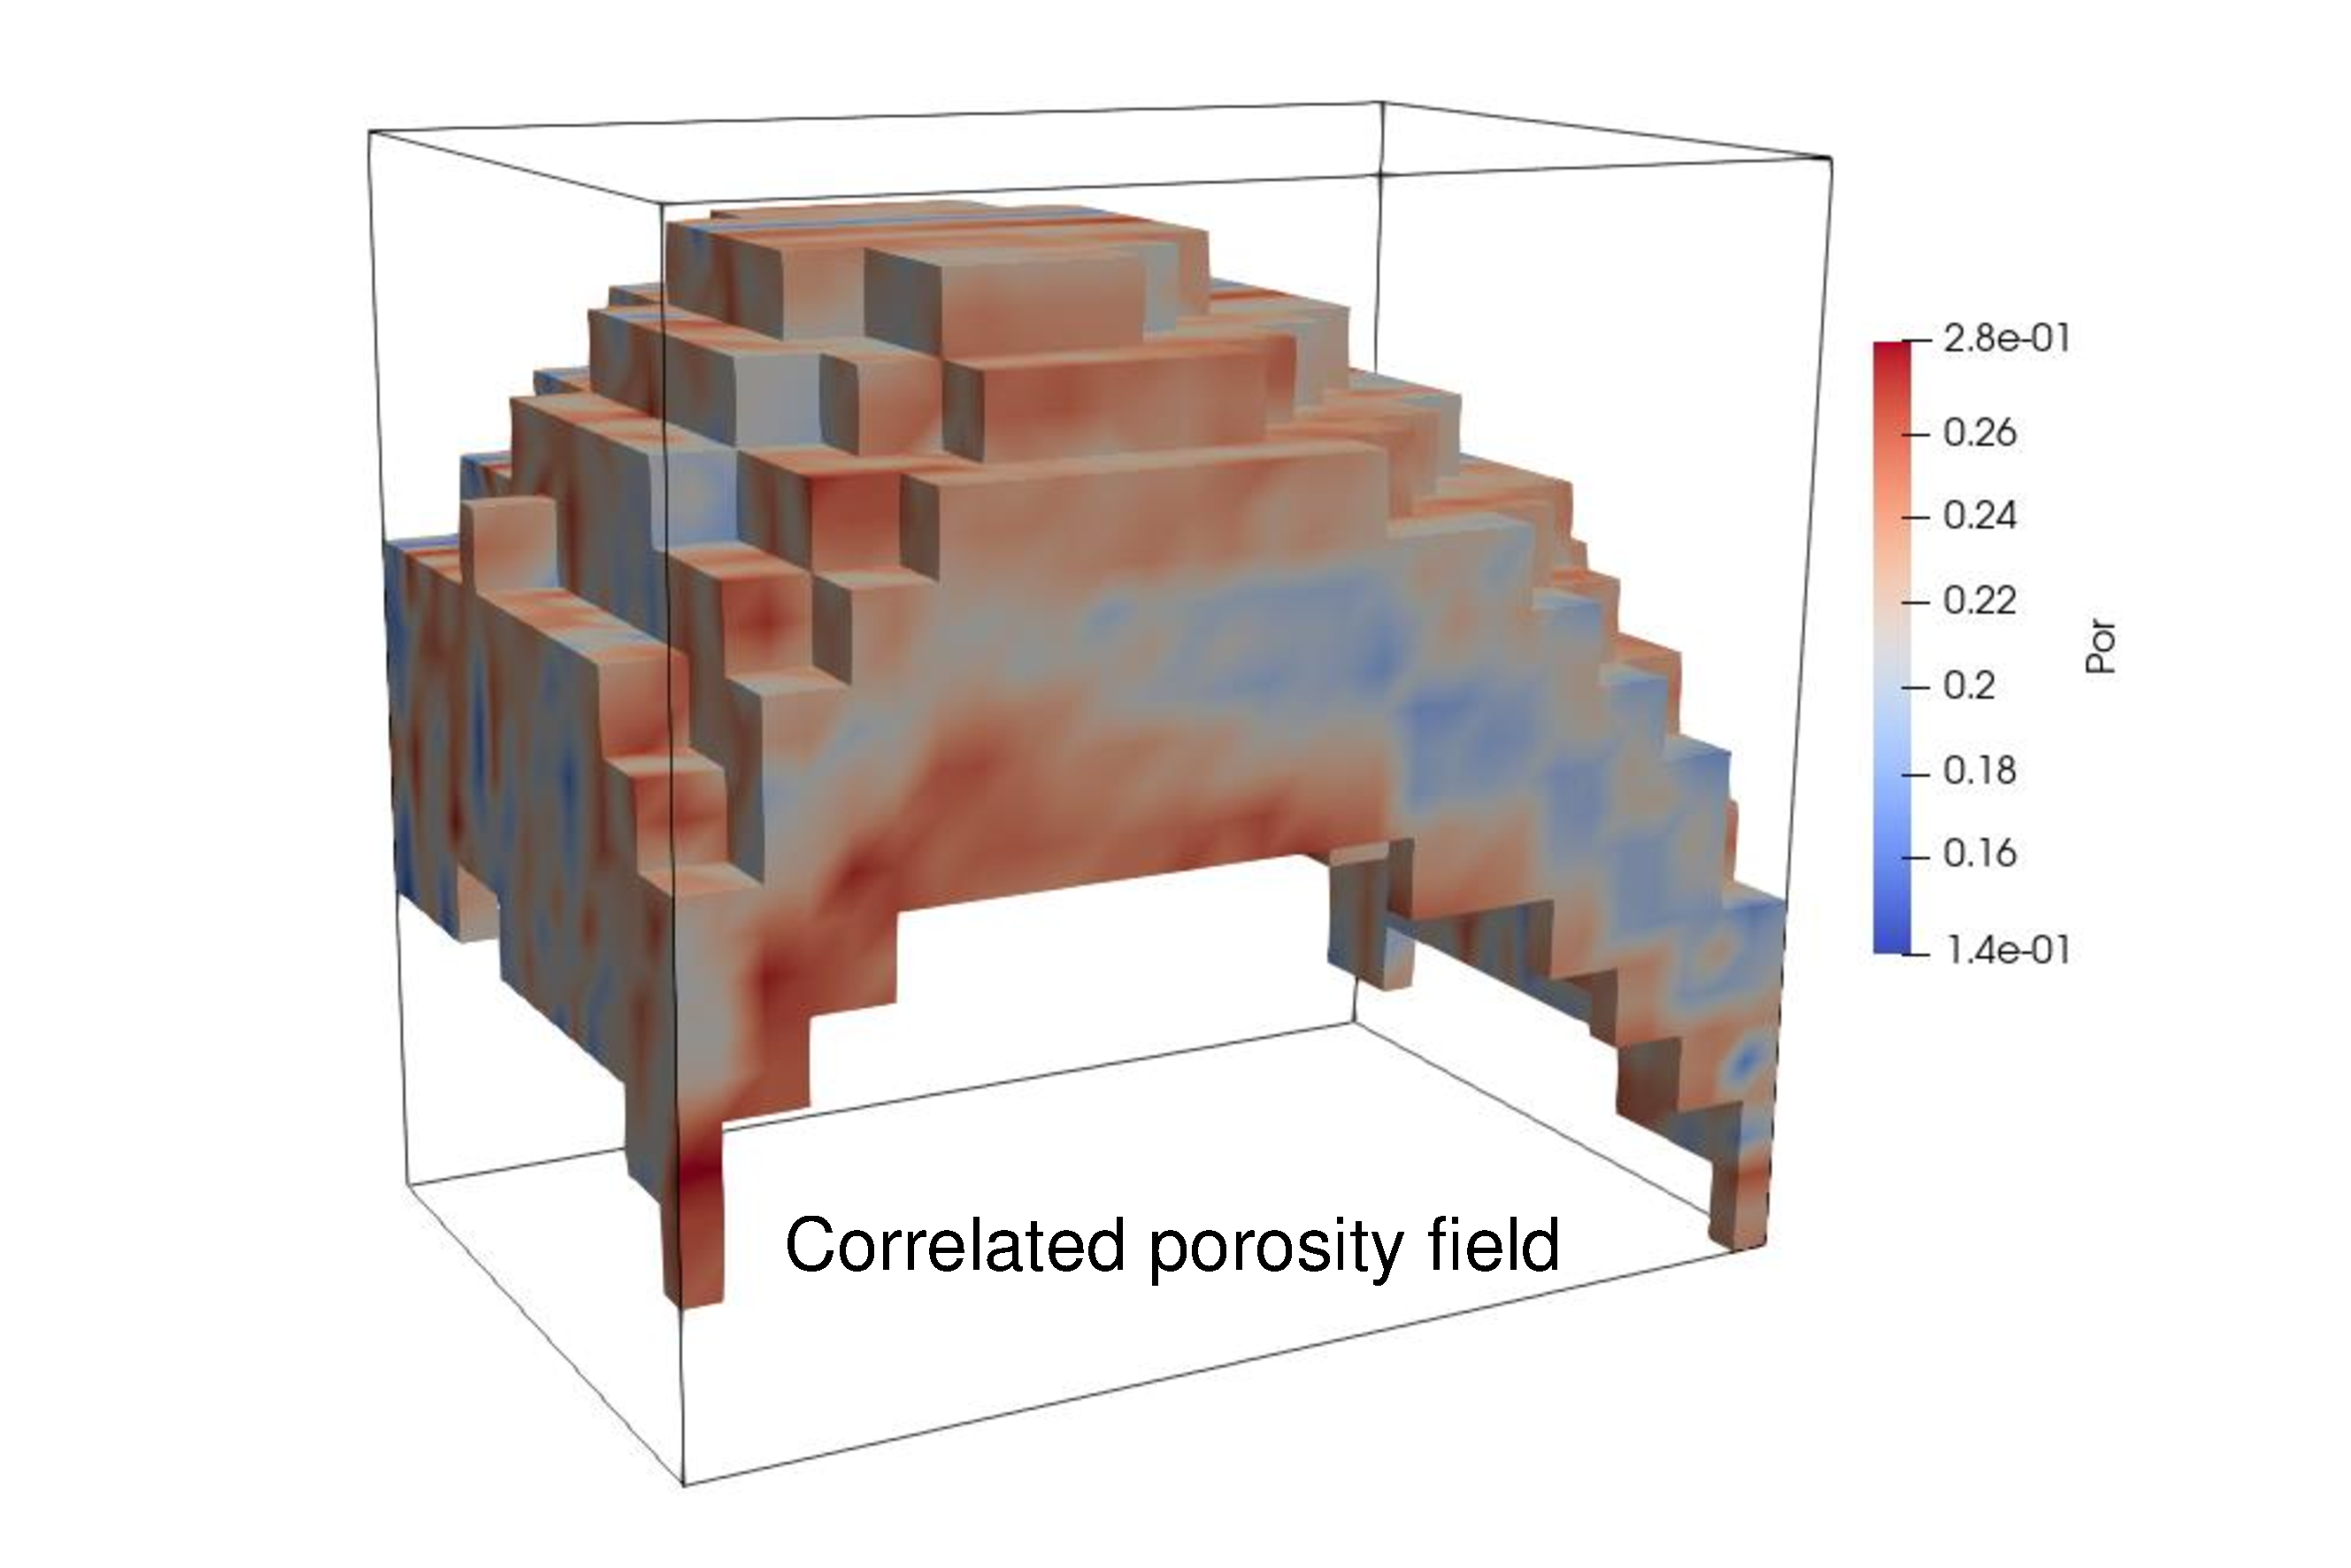
\includegraphics[width=0.8\textwidth]{Figures/porosity.pdf}}
    \caption{The correlated porosity field in fine-scale grid}\label{porosity}
\end{figure}

\begin{figure}[H]
    \centering    \centerline{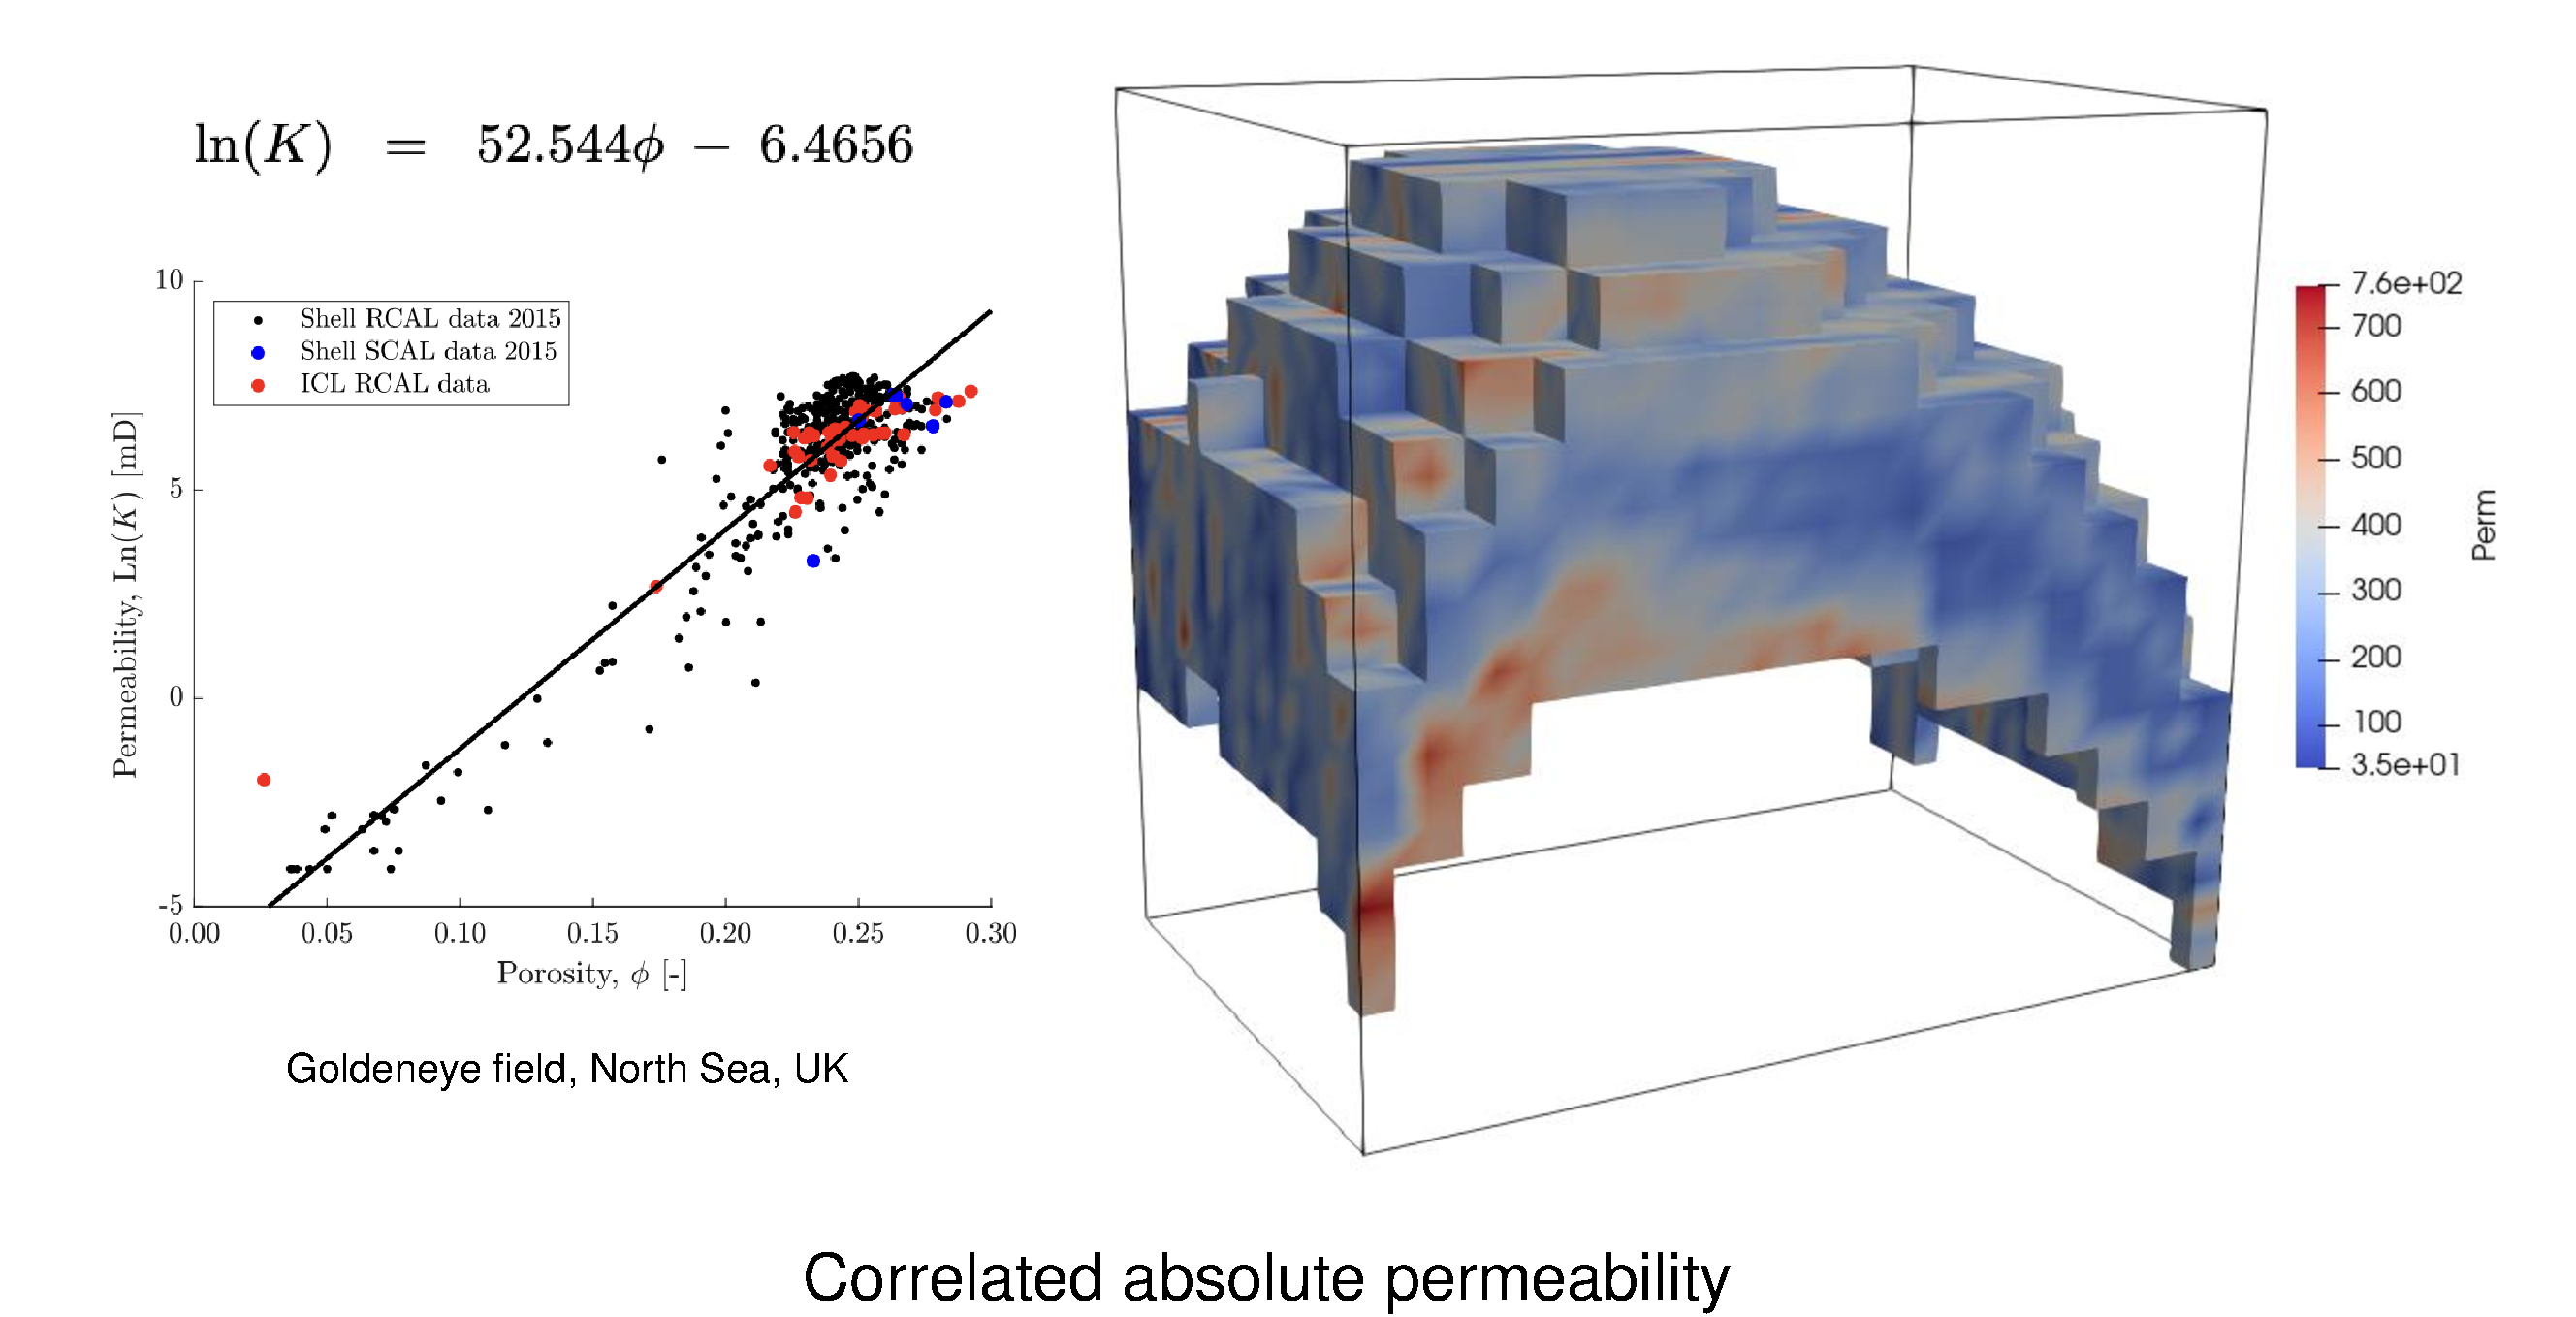
\includegraphics[width=1.1\textwidth]{Figures/Permeability.pdf}}
    \caption{The correlated absolute permeability field in fine-scale grid}\label{Permeability}
\end{figure}

\begin{figure}[H]
    \centering    \centerline{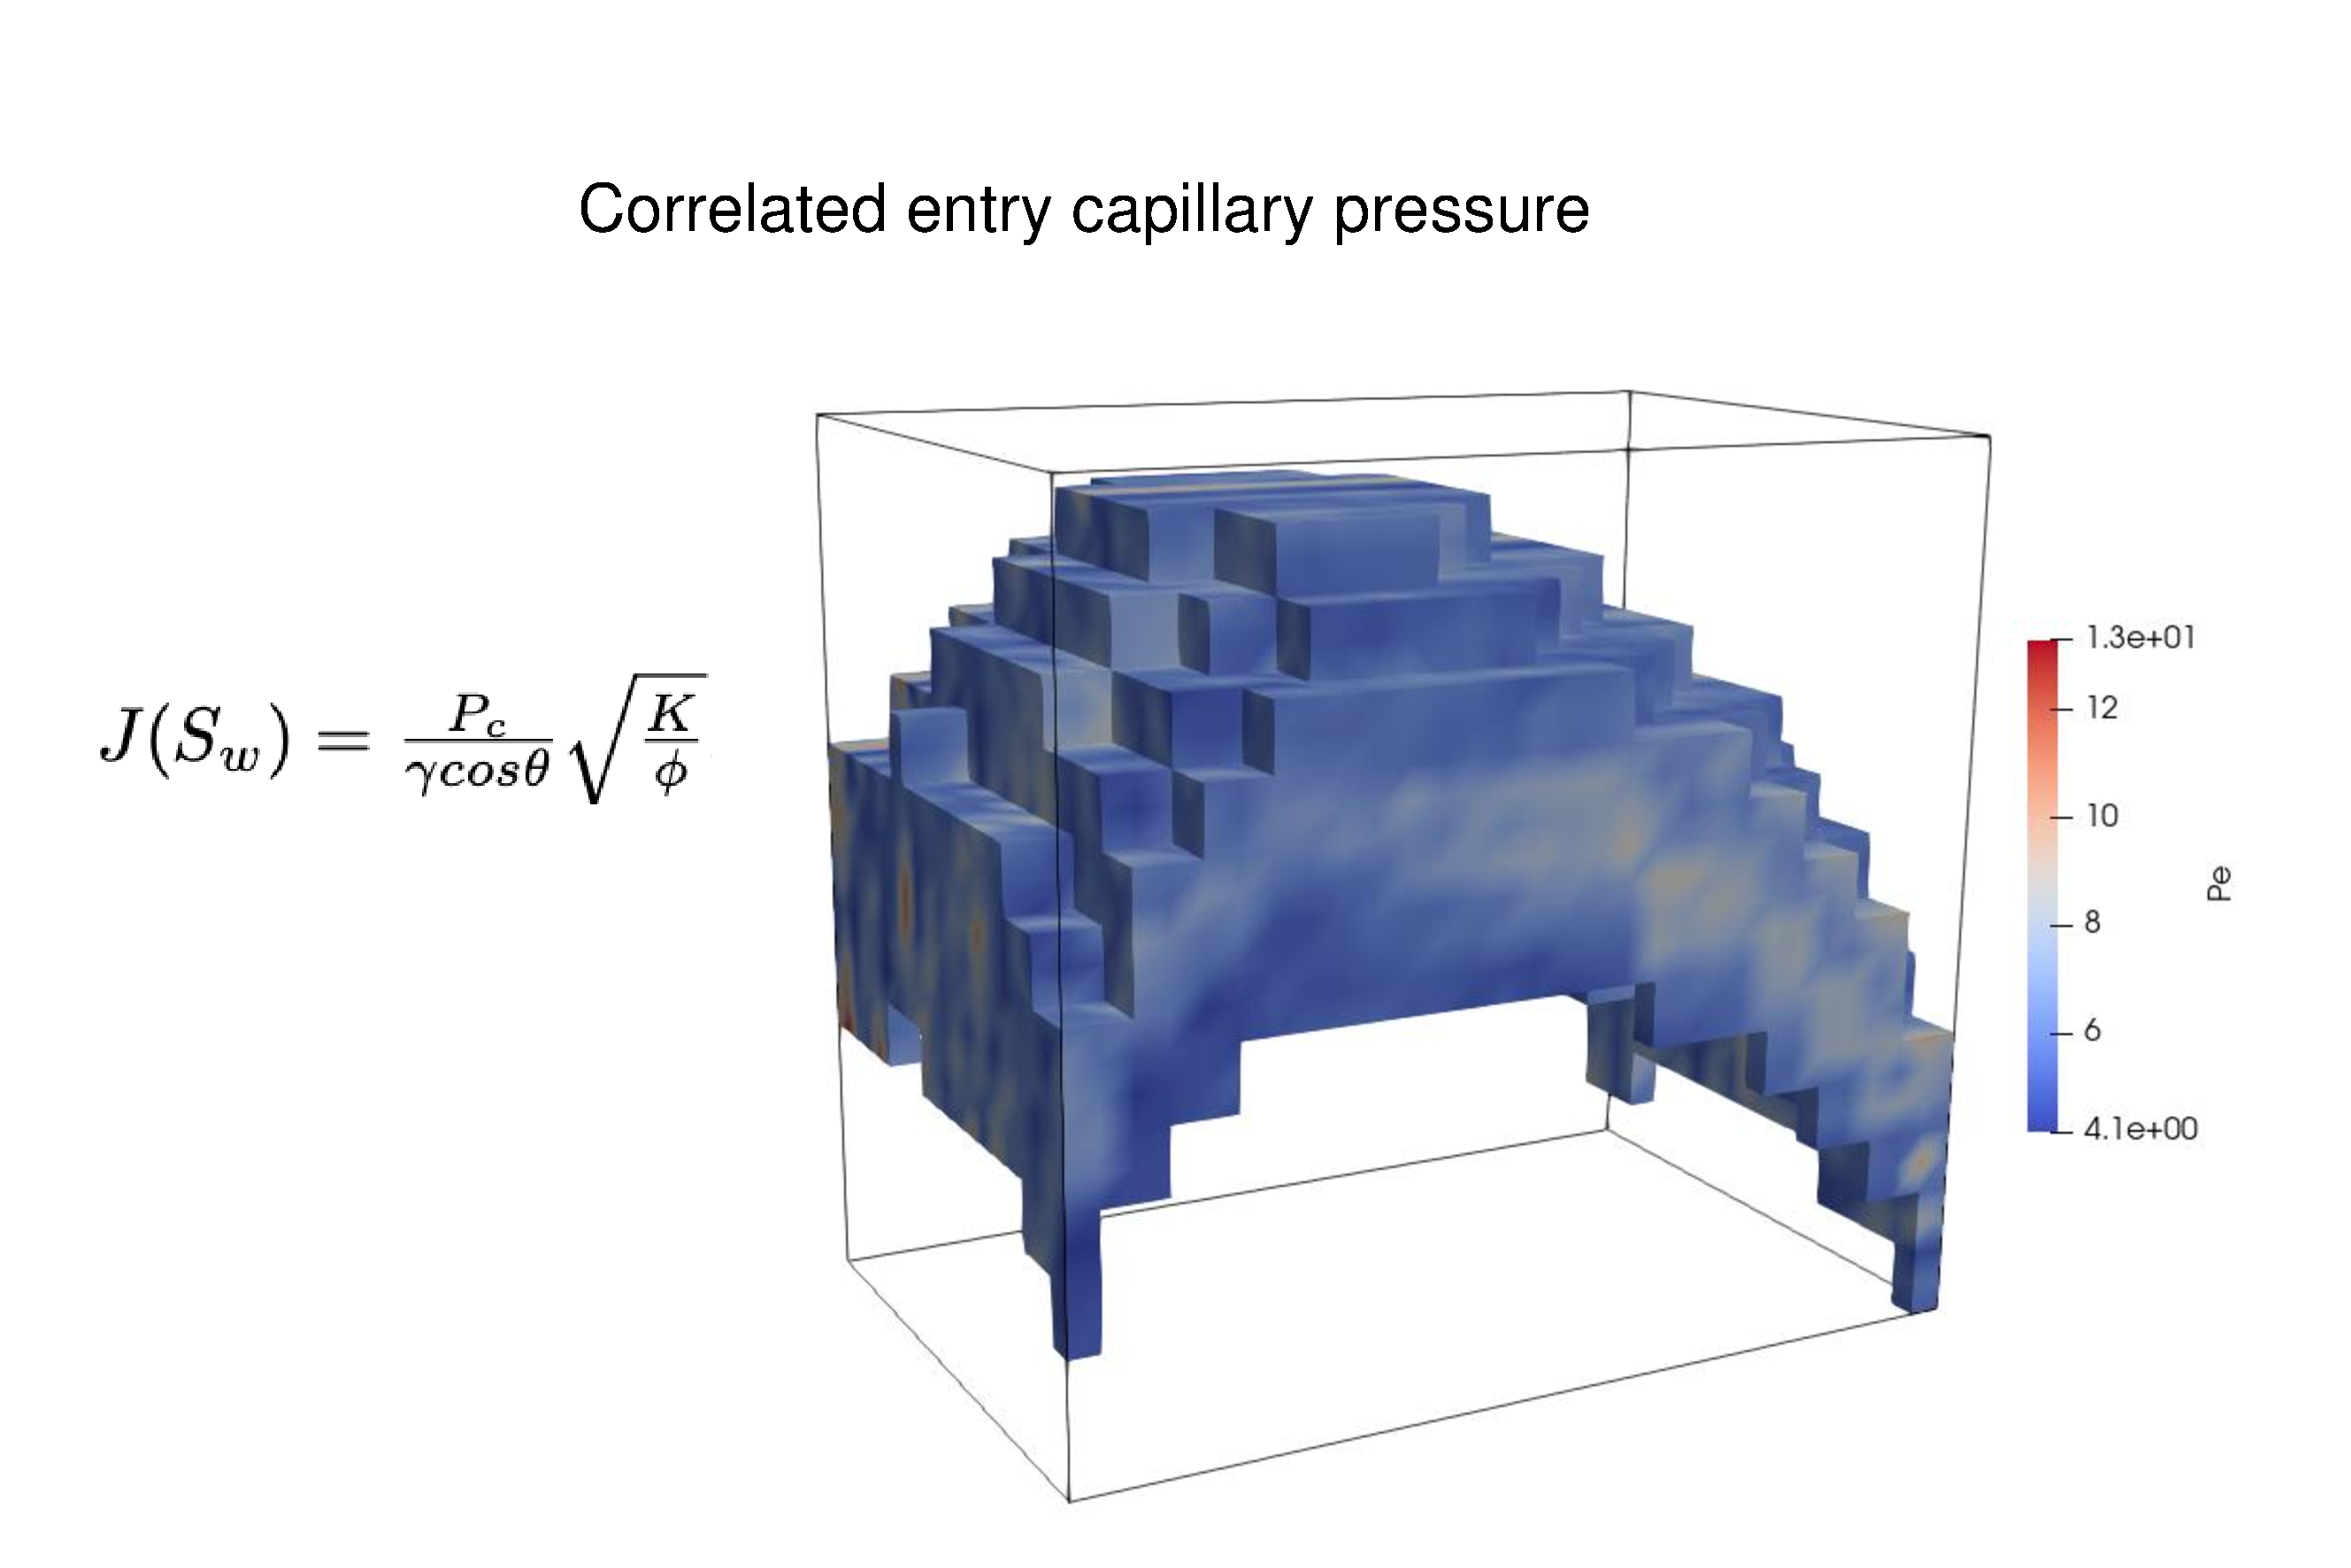
\includegraphics[width=0.8\textwidth]{Figures/Pe.pdf}}
    \caption{The correlated absolute permeability field in fine-scale grid}\label{Pe}
\end{figure}

\begin{figure}[H]
    \centering    \centerline{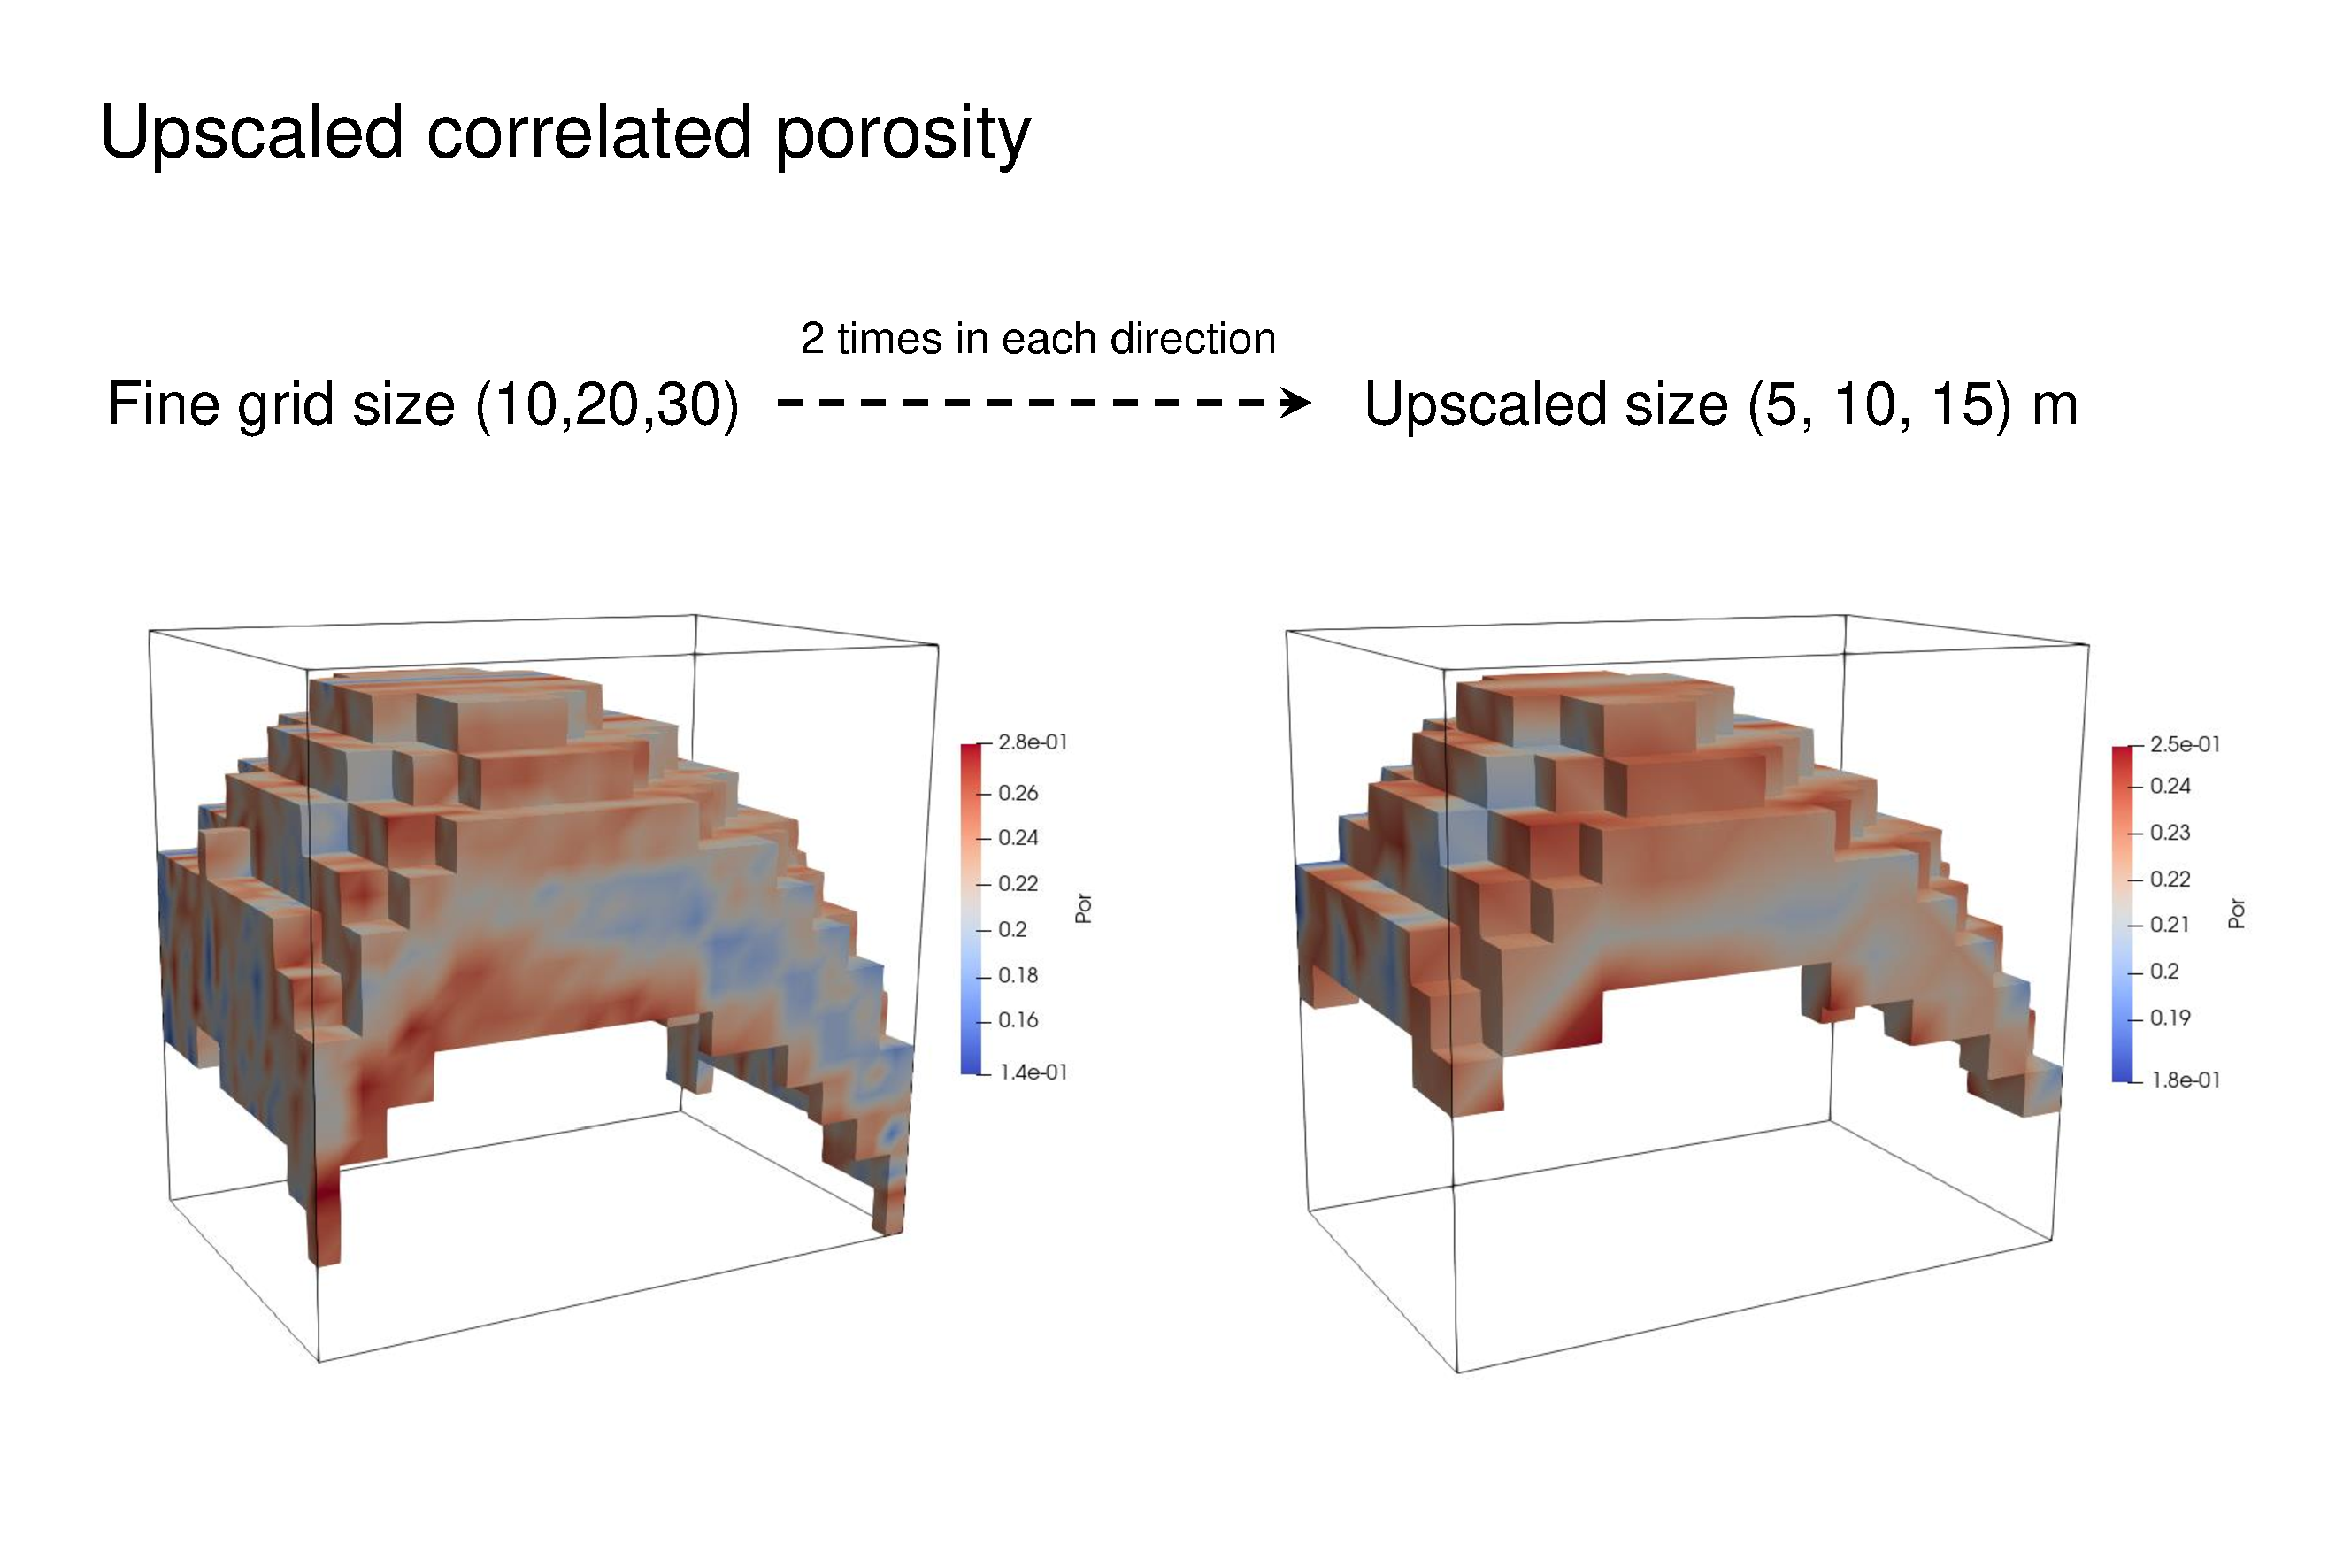
\includegraphics[width=1\textwidth]{Figures/porosity2.pdf}}
    \caption{The upscaling of correlated porosity field}\label{porosity2}
\end{figure}

\begin{figure}[H]
    \centering    \centerline{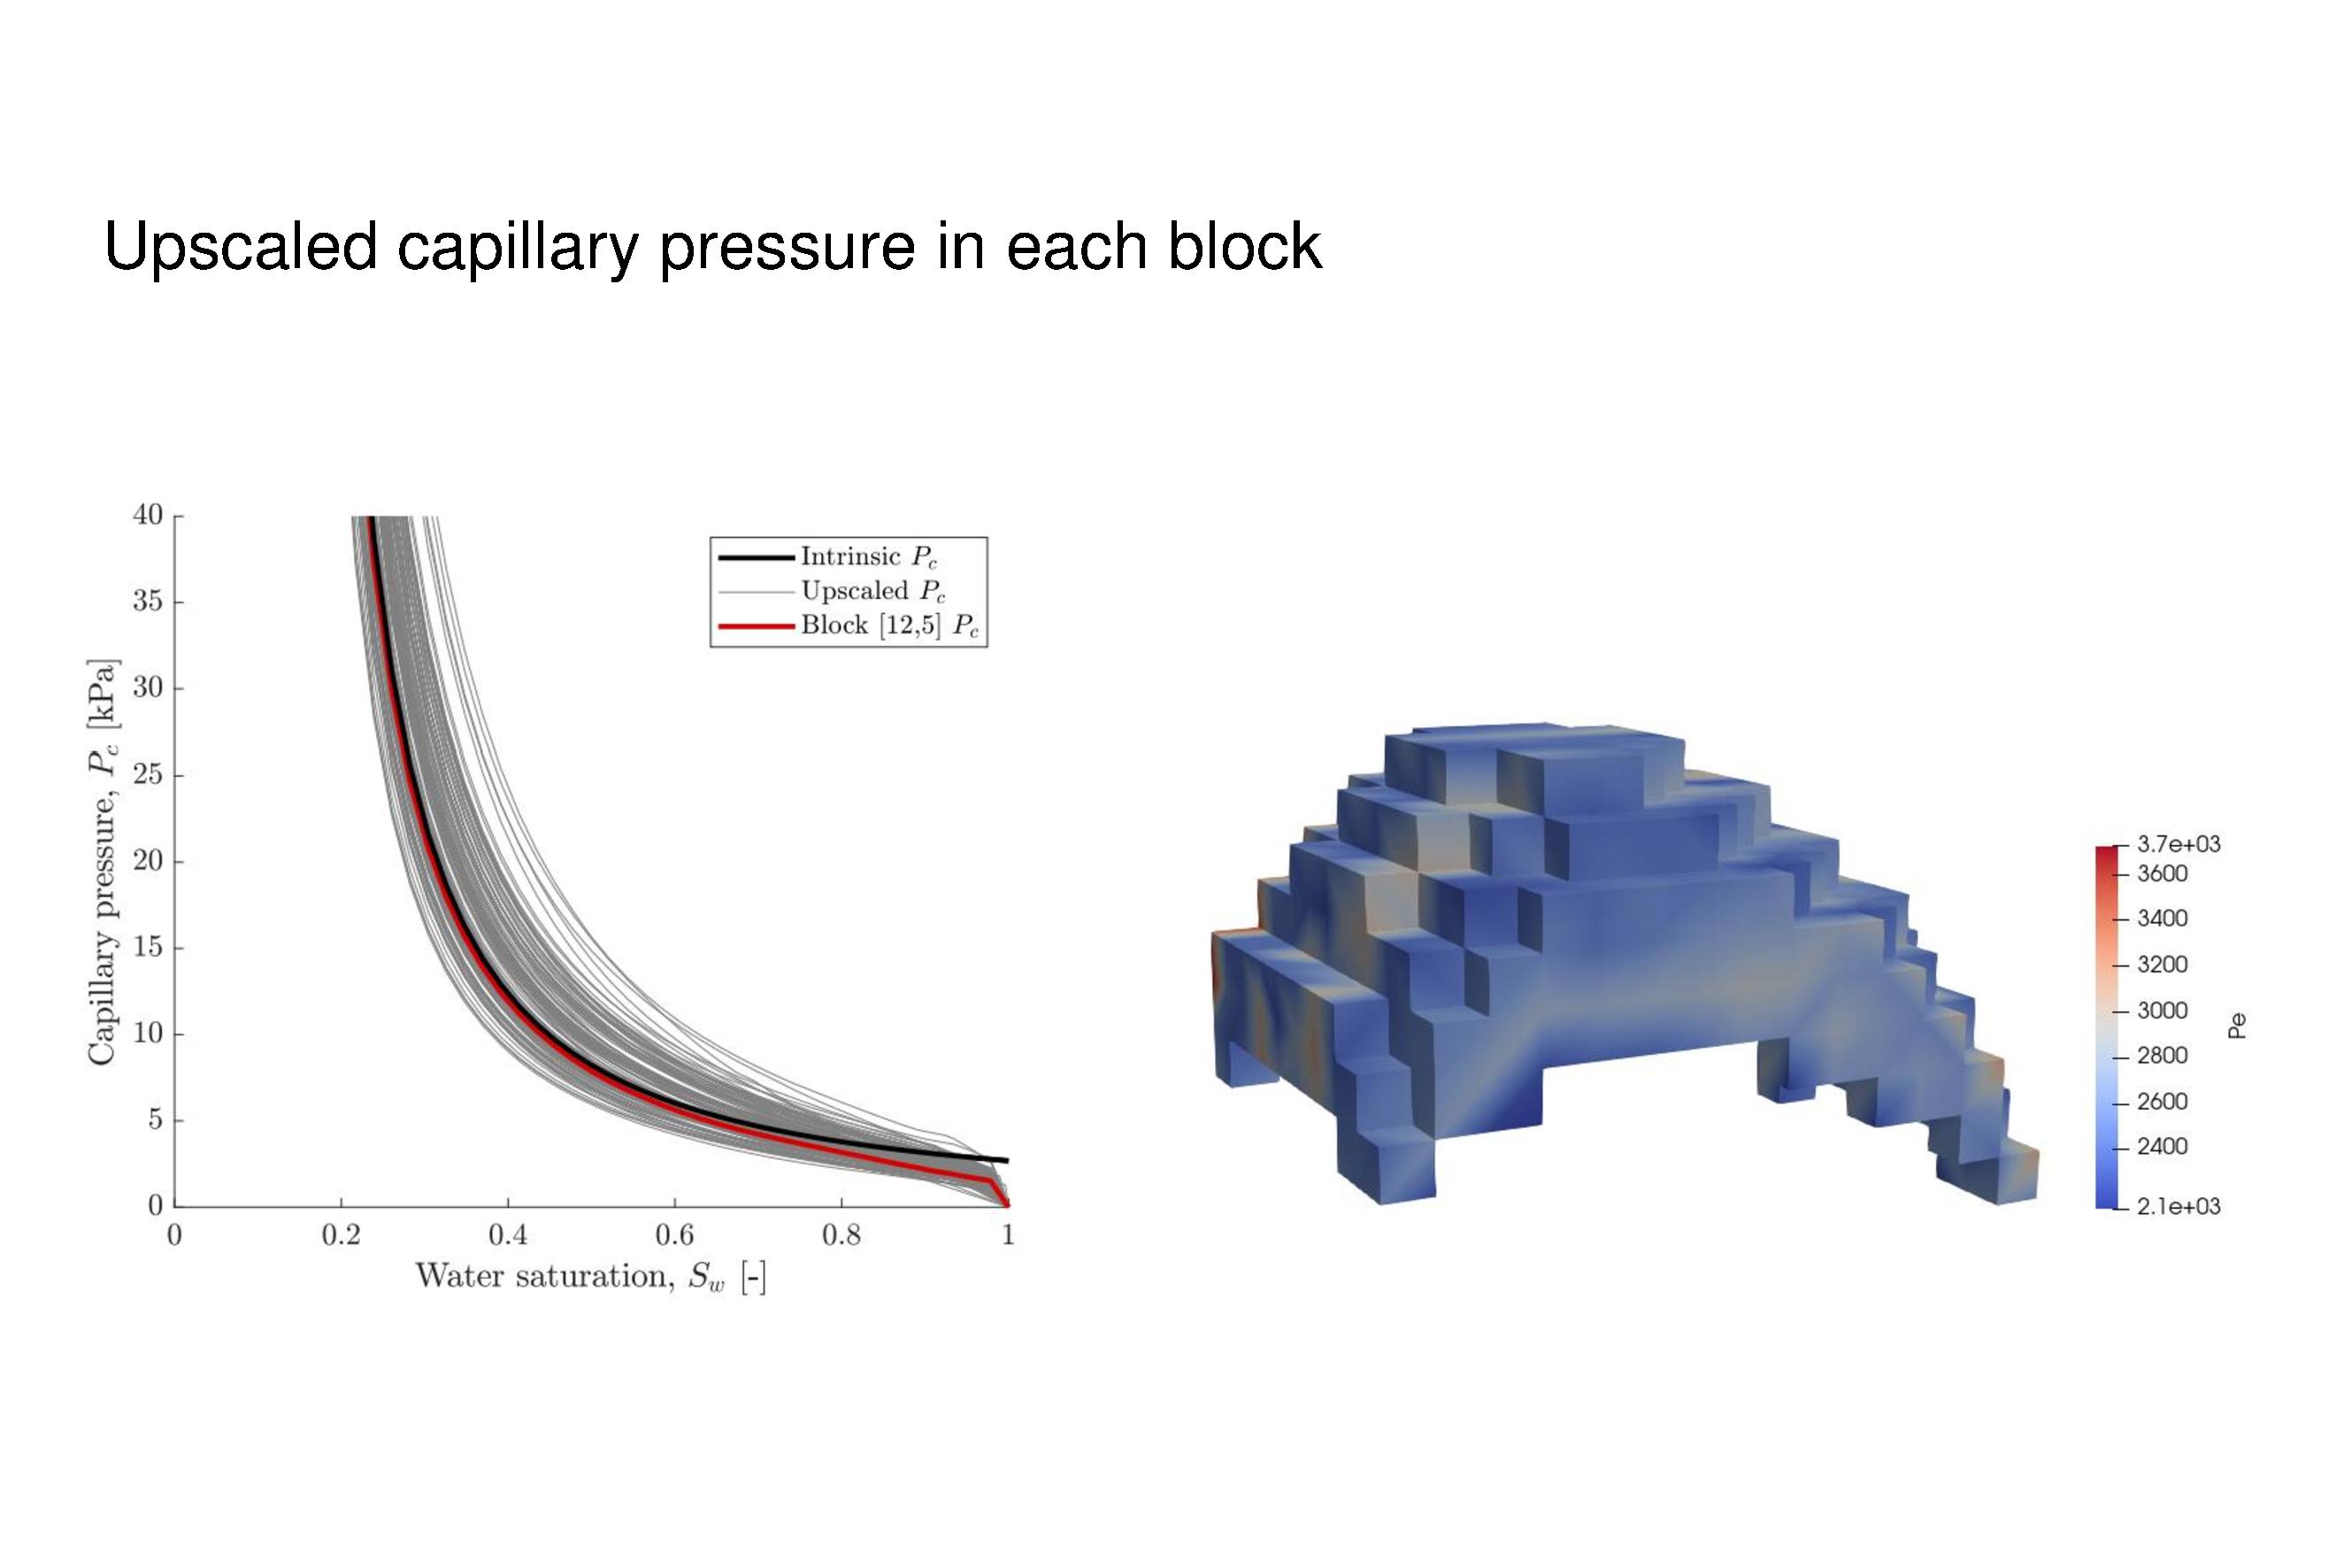
\includegraphics[width=1\textwidth]{Figures/Pe2.pdf}}
    \caption{Upscaled capillary pressure curve in each block}\label{Pe2}
\end{figure}

\begin{figure}[H]
    \centering    \centerline{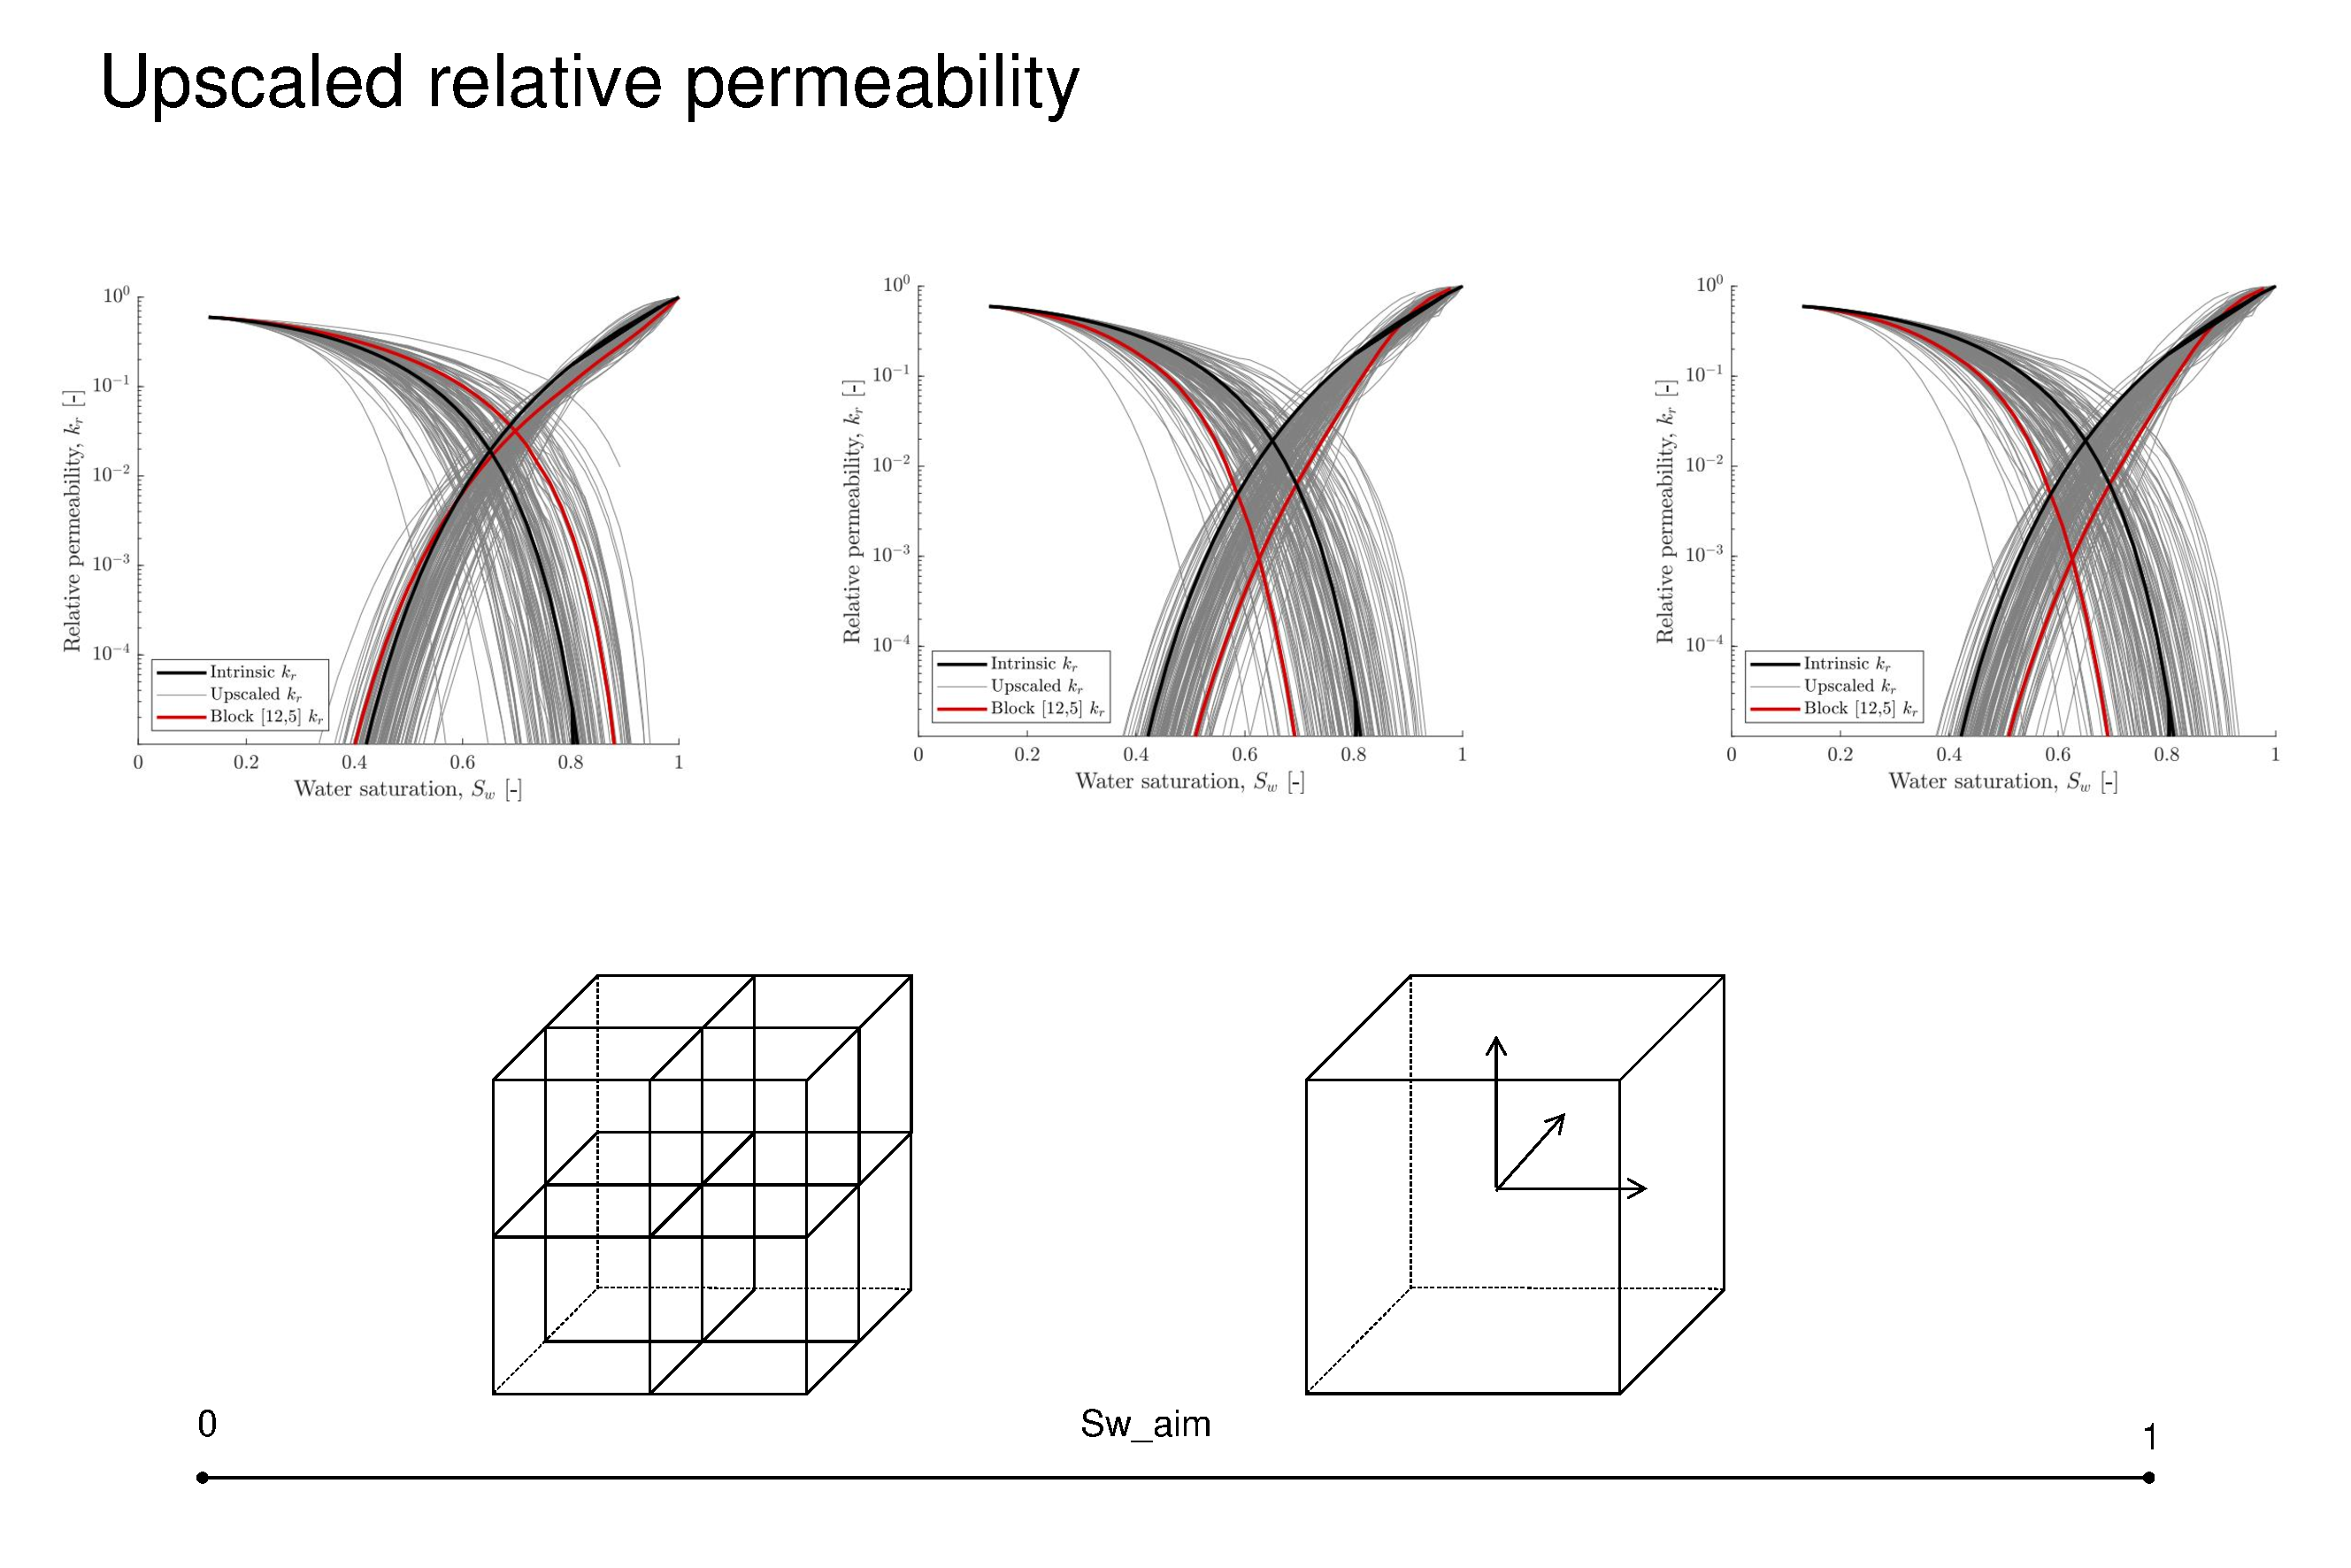
\includegraphics[width=0.8\textwidth]{Figures/Permeability2.pdf}}
    \caption{Directionally upscaled relative permeability in coarsen cells}\label{Permeability2}
\end{figure}

\nocite{*}

\section*{Acknowledgements}
We gratefully acknowledge funding from the Shell Digital Rocks II programme at Imperial College London.

\section*{Data Availability}
The readers can find the input data and raw data of figures presented in the manuscript in the Mendeley repository with the doi: 10.17632/5rcpb43g4w.2.

\bibliographystyle{ieeetr}
\bibliography{reference}

\end{document}
